\section{Hybrid AC/DC and Converter-Limit Model}\label{sec:model}

\subsection{Network variables and nodal balances}

Let $\mathcal N_{\ac}$ and $\mathcal N_{\dc}$ denote the energized ac and dc
buses, and let $\mathcal C$ denote the supported limited VSCs. The network
state is
\begin{equation}
 x=(\theta,V,V_{\dc}),
\end{equation}
with only the coordinates required by the selected bus equations retained.
In a conventional grid-connected component, one terminal angle is omitted or
fixed. In a slackless GFM island, all terminal voltage magnitudes and angles
remain variables; a fixed internal GFM phasor supplies the absolute reference
through the device equation.

For ac bus $i$, the calculated complex injection is
\begin{equation}
 S_i^{\mathrm{net}}(V,\theta)
 =V_i e^{\mathrm j\theta_i}
  \overline{\sum_{k\in\mathcal N_{\ac}}
  Y_{ik}V_k e^{\mathrm j\theta_k}}.
\end{equation}
The active- and reactive-power residuals are written in the production
``specified minus calculated'' convention,
\begin{subequations}\label{eq:ac-balances}
\begin{align}
 F_{P,i} &= P_i^{\mathrm{spec}}(x,z)-\Re(S_i^{\mathrm{net}}),\\
 F_{Q,i} &= Q_i^{\mathrm{spec}}(x,z)-\Im(S_i^{\mathrm{net}}).
\end{align}
\end{subequations}
For dc bus $j$, with conductance matrix $G_{\dc}$,
\begin{equation}
 F_{\dc,j}=P_{\dc,j}^{\mathrm{spec}}(x,z)
 -V_{\dc,j}(G_{\dc}V_{\dc})_j.
 \label{eq:dc-balance}
\end{equation}
Each converter contributes its explicit $(P_{\ac,c},Q_{\ac,c},P_{\dc,c})$
directly to the corresponding nodal balances. This ownership is important:
converter power, limit activity, and internal-voltage results are solver
variables and certificates, not values inferred after convergence from a bus
net injection.

\subsection{Fixed local converter state}

Every $c\in\mathcal C$ owns the six-state vector in
\eqref{eq:local-state-intro}. The complete nonlinear system is
\begin{equation}
 H(w)=0,\qquad
 w=(x,z_1,\ldots,z_m),\quad m=|\mathcal C|,
 \label{eq:complete-system}
\end{equation}
where $H$ stacks the network balances and six local equations per converter.
The local state has one meaning across steady power flow, quasi-steady replay,
OPF post-processing, and transient initialization. For non-GFM power-port
modes, $E_{r,c}=E_{i,c}=0$ are identity equations; the slots are retained so
the dimension and sparse coordinates do not change with control role.

\subsection{Power command and dc-voltage droop saturation}

For PQ operation,
\begin{equation}
 P_c^{\mathrm{ref}}=P_c^{\mathrm{set}},\qquad
 Q_c^{\mathrm{ref}}=Q_c^{\mathrm{set}}.
\end{equation}
For Vdc-Q operation, the active-power command is
\begin{subequations}\label{eq:vdc-droop}
\begin{align}
 P_c^{\mathrm{raw}}
 &=k_{v,c}\left(V_{\dc,c}^{2}-(V_{\dc,c}^{\mathrm{set}})^2\right),\\
 P_c^{\mathrm{ref}}
 &=\clip(P_c^{\mathrm{raw}},P_c^{\min},P_c^{\max}),\\
 Q_c^{\mathrm{ref}}&=Q_c^{\mathrm{set}}.
\end{align}
\end{subequations}
Inside the open unsaturated interval,
$\partial P_c^{\mathrm{ref}}/\partial V_{\dc,c}=2k_{v,c}V_{\dc,c}$;
outside it the derivative is zero. The power bounds are therefore represented
inside the local equations rather than through an external mode switch.

\subsection{Current disk and power-port priorities}

For terminal voltage magnitude $V_c$ and current limit $I_c^{\max}$, define
\begin{equation}
 R_c=V_c I_c^{\max},\qquad
 g_c=R_c^2-P_{\ac,c}^2-Q_{\ac,c}^2.
 \label{eq:current-disk}
\end{equation}
The magnitude-priority model radially scales the requested complex power:
\begin{subequations}\label{eq:magnitude-priority}
\begin{align}
 (1+\lambda_c)P_{\ac,c}-P_c^{\mathrm{ref}}&=0,\\
 (1+\lambda_c)Q_{\ac,c}-Q_c^{\mathrm{ref}}&=0,\\
 \phi_{\mathrm{FB}}(\lambda_c,g_c)&=0,
\end{align}
\end{subequations}
where
\begin{equation}
 \phi_{\mathrm{FB}}(a,b)=\sqrt{a^2+b^2}-a-b.
 \label{eq:fb}
\end{equation}
Equation~\eqref{eq:fb} is zero exactly when
$a\ge0$, $b\ge0$, and $ab=0$.

For P-first and Q-first operation, define the median projection residual
\begin{equation}
 \mathcal M(y;r,\ell,u)
 =\max\!\left(\min(y-r,y-\ell),y-u\right).
 \label{eq:median}
\end{equation}
The equation $\mathcal M=0$ returns the reference when it is feasible and the
nearest bound otherwise. P-first operation is
\begin{subequations}\label{eq:p-first}
\begin{align}
 \mathcal M(P_{\ac,c};P_c^{\mathrm{ref}},-R_c,R_c)&=0,\\
 R_{Q,c}&=\sqrt{\max(0,R_c^2-P_{\ac,c}^2)},\\
 \mathcal M(Q_{\ac,c};Q_c^{\mathrm{ref}},-R_{Q,c},R_{Q,c})&=0,\\
 \lambda_c&=0.
\end{align}
\end{subequations}
Q-first operation exchanges $P$ and $Q$ in \eqref{eq:p-first}. A finite
selected generalized derivative is used when the remaining radius is zero.

Figure~\ref{fig:priority-geometry} shows the geometric distinction among the
three policies for one normalized infeasible request. Magnitude limiting moves
radially to the current circle. P-first retains the feasible active component
before assigning the remaining reactive radius, whereas Q-first performs the
dual construction. The figure is an equation-level illustration; measured
production results are reported separately in Section~\ref{sec:preliminary}.

\begin{figure*}[t]
\centering
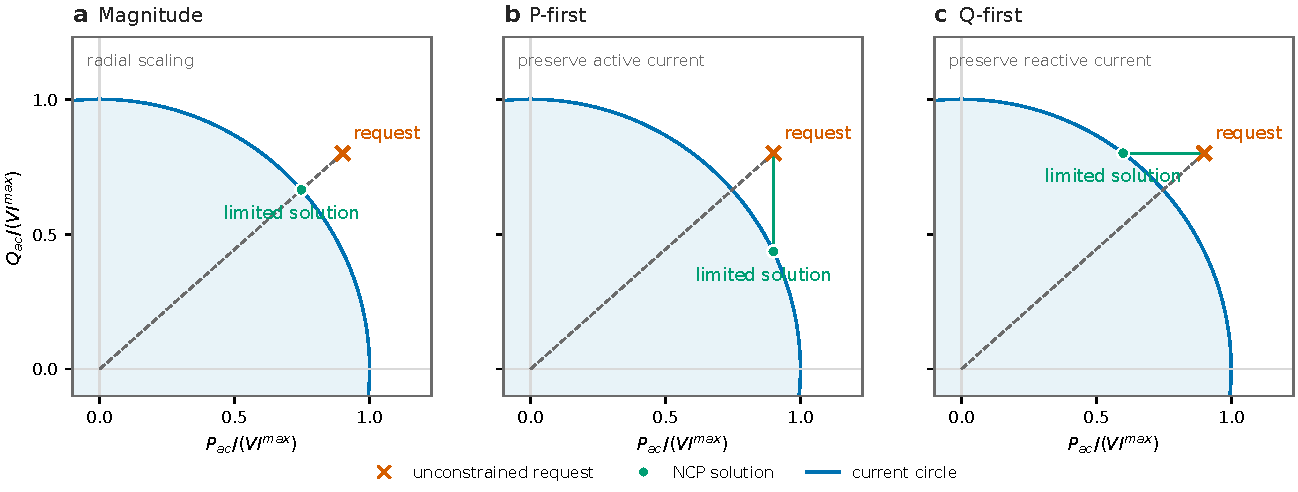
\includegraphics[width=0.92\textwidth]{figures/priority_geometry.pdf}
\caption{Normalized current-circle geometry for the common infeasible request
$(P^{\mathrm{ref}},Q^{\mathrm{ref}})/(VI^{\max})=(0.9,0.8)$. The orange cross
is the unconstrained command and the green point is the NCP solution.
(a) Magnitude priority scales both components radially. (b) P-first preserves
active current and clips reactive current to the remaining radius. (c) Q-first
preserves reactive current and clips active current.}
\label{fig:priority-geometry}
\end{figure*}

All power-port priorities close converter energy balance through
\begin{equation}
 P_{\dc,c}+P_{\ac,c}
 +P_c^{\mathrm{loss}}(P_{\ac,c},V_{\dc,c})=0,
 \label{eq:energy-balance}
\end{equation}
with analytic derivatives from the selected production loss model.

\subsection{Grid-forming Norton equation family}

Let
\begin{equation}
 \mathcal V_c=V_c e^{\mathrm j\theta_c},\quad
 E_c=E_{r,c}+\mathrm jE_{i,c},\quad
 Z_{v,c}=R_{v,c}+\mathrm jX_{v,c}.
\end{equation}
The converter current and terminal power are
\begin{equation}
 I_c=\frac{E_c-\mathcal V_c}{Z_{v,c}},\qquad
 S_{\ac,c}=\mathcal V_c\overline{I_c}
 =P_{\ac,c}+\mathrm jQ_{\ac,c}.
 \label{eq:gfm-port}
\end{equation}
Thus the first two local equations enforce the real and imaginary parts of
\eqref{eq:gfm-port}, and \eqref{eq:energy-balance} supplies the third.

For magnitude limiting, let $E_c^0$ be the authored internal-voltage reference.
The remaining equations are
\begin{subequations}\label{eq:gfm-magnitude}
\begin{align}
 (1+\lambda_c)(E_c-\mathcal V_c)
 -(E_c^0-\mathcal V_c)&=0,\\
 \phi_{\mathrm{FB}}\!\left(
 \lambda_c,(I_c^{\max})^2-|I_c|^2\right)&=0.
\end{align}
\end{subequations}
The complex equation in \eqref{eq:gfm-magnitude} supplies two real rows. It can
be interpreted as an implicit increase in the virtual impedance when the
current circle becomes active.

For P-first and Q-first GFM limiting, $I_c$ and the unconstrained current
$I_c^0=(E_c^0-\mathcal V_c)/Z_{v,c}$ are rotated into the terminal-voltage synchronous
frame. The primary current component is projected onto
$[-I_c^{\max},I_c^{\max}]$ using \eqref{eq:median}; the secondary component is
projected onto its remaining circular radius. The unused multiplier is fixed
by $\lambda_c=0$. This construction preserves the same six rows and variables
for all three priorities.

\subsection{Model scope}

The equations describe a balanced positive-sequence steady or quasi-steady
operating point after limit activation. They do not represent PWM switching,
the fast current-control transient, or EMT fault dynamics. A GFM terminal in a
slackless island retains its terminal $V/\theta$ variables and both nodal power
balances. The authored internal phasor $E_c^0$ breaks the global rotational
null mode through \eqref{eq:gfm-port}; no artificial terminal slack is added.
Multiple fixed Norton sources can coexist, with power sharing and circulating
power determined by their phasors and virtual impedances.
